\chapter{Argumentation Mining}
\label{chap:argmin}

The area of argumentation mining is a relatively new field established as a
subarea of computational linguistics.  At the time of the writing, there have
been seven workshops and two tutorials co-located with top ranked computational
linguistics conferences,\footnote{According to Google Scholar
\url{https://scholar.google.com} and Conference Ranks
\url{http://www.conferenceranks.com/}} all within the past five years. The
growth can largely be attributed to the advent of robust natural language
processing methods and the increased availability of argumentative data sources,
such as internet debates and discussions. 

In this chapter, first we will explain the research scope argumentation
mining and give a short overview of its history (Section~\ref{sec:definition}).
Then, a systematic summary of argumentation mining tasks is provided
(Section~\ref{sec:problems}). Applications and corpora for argumentation mining 
are listed in Section~\ref{sec:applications}. 
Finally, we reflect on criticisms of argumentation mining
and position this thesis within current research on argumentation mining
(Section~\ref{sec:area_discussion}).

\section{Definition}
\label{sec:definition}

\begin{figure}[t]
	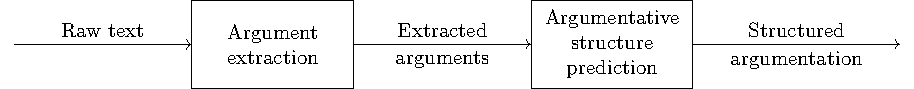
\includegraphics{area_description_pipeline-figure0.pdf}
	\caption{Pipeline architecture of an end-to-end argumentation mining 
	system}
	\label{fig:pipeline}
\end{figure}

\emph{Argumentation mining} is a discipline dealing with the automatic
identification and extraction of the structure of inference and reasoning
expressed as arguments presented in natural language
\citep{lawrence2019argument}.  Some refer to it as argument mining; we will use
both names interchangeably.  Argumentation mining combines elements of
\emph{natural language processing} (discussed briefly in
section~\ref{sec:natural_language_processing}) and \emph{knowledge
representation and reasoning} \citep{cabrio2018five}.  Typically, natural
language processing techniques are first used to extract arguments and
structure a debate or discussion. Then, once the argumentative parts of a
debate or discussion have been extracted and structured, they are provided as
input to knowledge representation and reasoning systems.  Knowledge
representation and reasoning systems are usually in charge of providing various
argumentation analysis, examples being: determining stance,
detecting logical fallacies, or finding most frequently used claims.

To get from raw text to structured arguments, a pipeline-like architecture
is usually employed (shown in Figure~\ref{fig:pipeline}). 
Raw (natural language) text is input to an argument extraction module. This module
extracts elementary \textbf{argument components} from raw text. 
Once argument components are extracted, they are connected and structured 
according to some \textbf{argumentation model} (such as the Toulmin model \citep{toulmin2003uses}).
The output of the structuring module is usually some form of an argument graph. 
%An alternative, but similar architecture is shown
%in~\citep{lippi2016argumentation} where the argument extraction component 
%is elaborated further. 
In this thesis, we will mostly discuss extracting and structuring argumentative
portions of a textual debate. We will briefly showcase how a analysis can be
conducted in Chapter~\ref{chap:analysis}. 

\subsection{Example}


Fig.~\ref{fig:example_pipeline} shows an example of an argumentation mining
pipeline. Two comments are taken from an internet discussion forum on the topic
of ``\emph{Should marijuana be legalized?}''. The author of the first comment
is \con{against} the legalization of marijuana, the author of the second
comment is \pro{for} the legalization of marijuana.  In this example, we use an
argument model that defines argument components to be premises and conclusions.
Premises and conclusions are singled out in the first step of the pipeline.
The second step of the pipeline detects relationships between extracted
argument components and forms argumentation structures. In this case, the
argumentation structure is defined by the Freeman's model
\citep{freeman2011argument}, which defines premises and conclusions with attack
or support relations amongst them. 

This example is from a dataset built by \citet{hasan2014you}. It demonstrates
some of the challenges of argumentation mining (and natural language processing
in general): the text contains typos (``\emph{nonsence}''), idiomatic
expressions (``\emph{because Marijuana is the drugs}''), requires solving
anaphora resolution to clarify context (``\emph{If you legalized, you could tax
it too}''), etc. All of these issues indicate that creating a coherent
argumentative logical structure from raw text is an extremely challenging
problem.

\begin{figure}[t!]
	\centering
	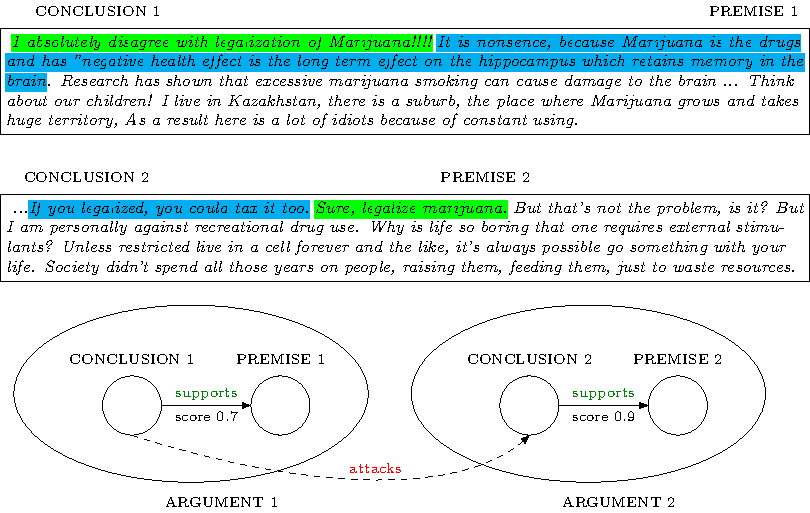
\includegraphics{area_description_example-figure0.pdf}
\caption{Example of two comments processed using an argumentation mining pipeline. 
	First, argument boundaries are determined for the \hlcyan{conclusions} and 
	\hlgreen{premises}. Then \textcolor{darkgreen}{support} and 
	\textcolor{red}{attack} relations are
	determined between conclusions and premises
	to form arguments.
	}
	\label{fig:example_pipeline}
\end{figure}

\subsection{History}

Argumentation has roots in dialectics and philosophy, where it was a branch of
knowledge dedicated to the study and analysis of how assertions are proposed
and debated, and how conflicts between opposing opinions are resolved
\citep{bench2007argumentation}.  Argumentation has been an essential part of
numerous areas, such as logic, rhetoric, jurisprudence, and computer science. 
Argumentation in computer science started with 
the work of \citep{dung1995acceptability}, who explored knowledge representation
of argumentation. Subsequent related work on argumentation
knowledge representation led to the development of 
the area now known as \emph{computational argumentation}. 

Computational argumentation studies three different types of models of argumentation:
rhetorical, dialogical, and monological \citep{bentahar2010taxonomy}. 
The two former highlight argumentation as a dynamic process: rhetorical models
put emphasis on the role of audience and persuasive intention; dialogical 
models describe the ways arguments are connected in a dialogical structure. 
The latter, monological models emphasize the structure of the argument itself, 
including the relations between different components of a given argument. 

Another dichotomy in computational argumentation is between 
\emph{abstract argumentation} and \emph{structured argumentation}, with
Dung as the main proponent of abstract argumentation \citep{dung1995acceptability,
bondarenko1997abstract}. In abstract argumentation, each argument is an
atomic entity without internal structure. Contrary to that, 
structured argumentation proposes some internal structure for each argument, 
described through some representation formalism or model. 
Argumentation mining typically follow the structured argumentation
school. In structured argumentation it is common to annotate text data according to
a defined (usually established on some argumentation theory) formalism, which is
then followed by building models to automatically derive argumentation
structure directly from text. There are many approaches in structured
argumentation, therefore there is no universally accepted definition of a
structured argument.  An intuitive definition of an argument was given by
\citet{walton1998new} as a statement consisting of three parts: a set of
premises, a conclusion, and inference from premises to a conclusion. However,
some literature (this thesis included) will denote premises and conclusions to
be referred to as claims.  What types of links can be established between
premises and conclusions (claims in general) varies greatly across different
argumentation models \citep{lippi2016argumentation}.

Independently of the development of computational argumentation and argumentation
mining, the area of \emph{opinion mining} (also referred to as sentiment
analysis) has developed as part of computational linguistics, especially in the
2000s. Opinion mining identifies the emotional tone of a body of text
\citep{pang2008opinion}.  It attempts to identify sentiment (positive, neutral,
or negative) and emotional state (happy, sad, angry, etc.) of the author of
the text.  Identifying opinions towards different (usually divisive) issues has
been researched as part of \emph{stance classification}
\citep{walker2012stance, hasan2013stance}.  Both sentiment analysis and stance
classification
are closely related to argumentation mining. In argumentation mining people
provide claims towards a topic. Their claims are usually backed up with arguments. These
arguments may contain subjective opinions (based on sentiment) and often result
in a final stance towards the topic of discussion (``\emph{gay marriages
should be allowed}''). In that light, argumentation mining often
(but not always) involves analyzing subjective opinion and stance. 

Argumentation mining started to become featured more prominently in the 2010s.
The work of \citet{teufel2009towards} is considered to be one of the first in
argumentation mining. They proposed argumentative zoning for scientific papers
in which they attempt to extract and structure argumentation on the paragraph
level.  \citet{palau2009argumentation} first started to work on a sentence
level, as they proposed an end-to-end solution to extract and structure
sentence-level arguments from legal texts. The development of machine learning
and natural language processing sparked further research and interest in
argumentation mining. Extensive research has then been conducted that mainly
adopted the \emph{structured argumentation} approach.

Within the scope of this thesis, we are interested in \emph{monological},
\emph{structured argumentation}.  We wish to analyze internet discussions without
accounting for the dialogical component, but merely the content of the
discussion. Structured argumentation is also the focus of our interest, as we
wish to grasp the semantics of arguments and claims, instead of treating them
as atomic units. Our structured argumentation approach is reflected in the fact that 
we decompose argumentative content into tokens, working our
way up to argument components. 

%- argumentation mining (often denoted as argument mining) started to gain dominance in 
%2010
%2010, when some of the 
%first methods to mine \textit{arguments} from natural language appeared in
%\citep{teufel2009towards} where they propose argumentative zoning for 
% scientific papers and \citep{palau2009argumentation} proposed to extract 
% and structure  arguments from legal texts. \\
%- development of machine learning and natural language processing sparked
%further research in the field of argumentation mining \\
%- since 2014 to 2019., there have been six argumentation mining dedicated workshops 
%co-located with top conferences in  computational linguistics (such as ACL and NAACL) \\
%- further, two seminars in Dagstuhl have been organized \\
%- two tutorials on argument mining have been held \\

% - One other definiton of argumentation mining states that
% it is  ``the general task of analyzing
% discourse on the pragmatics level and applying a  certain  argumentation  theory
% to  model  and  automatically analyze  the  data  at  hand'' \citep{habernal2017argumentation} \\
% 
% - argumentation mining spurned from people dealing with computational argumentation
% to develop more end-to-end methods \\

\section{Problems}
\label{sec:problems}

Two elementary problems of argumentation mining are 
extracting argument components from text and producing argumentative structure
from either extracted argument components or directly from text
(shown in Fig.~\ref{fig:pipeline}). 
Extracting argumentative components and producing argumentative
structure both make various assumptions about the data and downstream
applications. 
Extracting argumentative components from text is usually done in either
the sentence or paragraph level. Structuring arguments mostly adopts either 
Toulmin's or Freeman's model.
More specifically, problems in argumentation mining can
usually be specified by five dimensions \citep{lippi2016argumentation}: 
\begin{itemize}
\item \emph{granularity of input text}, 
\item \emph{genre of input text}, 
\item \emph{argument model}, 
\item \emph{granularity of output}, and
\item \emph{goal of analysis}.
\end{itemize}

\emph{Granularity of input text} indicates the detail at which arguments
are processed. Some process arguments at the paragraph level 
such as the work on argumentative zoning
\citep{teufel2009towards}. Most of current research defines
sentences as the minimal unit of argumentation,
whereas some authors explore the sub- and intra-sentence levels
to detect argument component boundaries.

\emph{Genre of the input text} is defined by the type of input data processed.
Usually, a single genre of documents is explored within an argumentation
pipeline, such as legal documents \citep{palau2009argumentation}, scientific
articles \citep{teufel2009towards}, or internet discussion forums
\citep{hasan2014you, boltuzic2014back, habernal2017argumentation}.  In
\citep{budzynska2014towards} they show how dialogue-agnostic and
context-agnostic models perform poorly.  Similar performance is shown in
\citep{daxenberger2017essence}, where they also attempt to design cross-genre
methods. Genre-specific research is explored more comprehensively in 
Section~\ref{sec:applications}.

Argumentation is structured through different \emph{argument models}.  The
argumentation model usually defines a formalism of argument components and
relationships between argument components.  Specific argument models are
described in Section~\ref{sec:area_arg_struc_pred}.

Similarly to the granularity of the input, the \emph{granularity of the output}
varies. The lowest possible granularity of output is a specific argument
component, such as claim, evidence, or premise. Argument components form arguments,
which are of more coarse granularity. Some even go beyond the level of arguments, 
and attempt to output \emph{argumentation schemes} \citep{feng2011classifying}, which
define the interactions across arguments, making them even coarser than arguments. 

Finally, the \emph{goal of analysis} describes the motivation behind solving
the argumentation mining problem. For typical argumentation mining problems
this can be (argument, claim) extraction, (argument component type)
classification, or (argument relation) prediction. An analyst can then 
summarize the discussion using the extracted claims, detect logical fallacies
of the extracted argumentation structure, etc.

Within the scope of this thesis, we will work on paragraph, sentence, and
sub-sentence \emph{granularity of input text}, with the emphasis on
sub-sentence level. We will define claims on a sub- and intra-sentence level as
part of the claim segmentation problem (Chapter~\ref{chap:claim_segmentation}).
The \emph{genre of input} will be, as the title suggests, internet discussions.
We define our own \emph{argumentation model} in
Chapter~\ref{chap:formalization} which is inspired by Freeman's model and the
work of \citet{hashimoto2012excitatory}.
The \emph{goal of analysis} of the thesis is claim extraction.
Next, we describe elementary problems of argumentation mining
argument component extraction and argumentative structuring 
in more detail.

% One example is the project of creating the
% Argument Web (argumentative Semantic Web) which defines knowledge
% representation standards for arguments compatible across different
% argumentation theories \citep{rahwan2007laying}. 

%- five dimensions of input are usually give: 
%granularity of input, genre of input, argument model, 
%granularity of target, goal of analysis \\
%- granularity of the processed text indicates  the detail at
%which arguments are processed \\
%- some consider argument processing at the level of paragraphs, 
%for example argument zoning \citep{teufel2009towards} \\
%- most of current research focuses on sentences, whereas some authors
%go to the intra-sentence level and detect argument component boundaries \\

% \noindent - the genre aspect defines the type of input data, such as legal/law, 
% internet discussions, news, essays, etc. \\
% - existing approaches have mainly considered a single genre \\
% - for example, \citep{budzynska2014towards} shows how AM need
% context, a dialogue-agnostic models do not work \\

% \noindent - tasks of argumentation mining are 
% \begin{itemize}
% \item prominent claim identification,
% \item claim clustering,
% \item claim extraction,
% \item deriving implied claims.
% \end{itemize}
% 
% \noindent - Argument extraction -- first step in identification of arguments
% within the input natural language text \\
% - may be further split per component extraction (claim/premise extraction) and
% by identification of text boundaries \\
% 
% \noindent - Relation prediction -- predicting what are the relations holding 
% between the arguments identified \\
% - the relations may heteregeneous, such as \emph{attack} and \emph{support}\\
% - upon their identification, these relations are used to connect arguments to 
% graphs, in which relations connecting the retrieved arguments (nodes of the graph)
% correspond to the edges \\

% \section{Argument analysis}
% 
% \noindent - manual argument analysis \citep{lawrence2019argument}
% - manual analysis often involves using various tools to analyze arguments, 
% such as Araucaria \citep{reed2004araucaria}, OVA \citep{reed2014ova+}, or
% Carneades \citep{gordon2007carneades} \\
% - these tools require already extracted claims that the tool users can then 
% connect, determine their roles (premise, conclusion) and define 
% relationships (attack, support), and even form refined structured,
% such as argumentation schemes \citep{walton2008argumentation} \\
% Generally, steps to perform argument analysis are:
% \begin{itemize}
% \item text segmentation,
% \item argument / non-argument,
% \item simple structure,
% \item refined structure.
% \end{itemize}

\subsection{Argument component extraction}
\label{subsec:arg_comp_ext}

The first stage of argumentation mining is detecting argumentative parts from
raw text.  There exists no standard for an elementary unit of argumentation,
but the definition is usually shaped to tailor a specific need. In discourse and
rhetoric theory, the basic element of an argument is called an \textit{Elementary
Discourse Unit} EDU. EDUs are defined as clauses \citep{winter1982towards,
givon1983topic}, sentences \citep{polanyi1996linguistic}, or 
prosodic units \citep{sacks1978simplest}. All these approaches agree an EDU
should be a non-overlapping atomic unit of text. Another strand of research defines
an \textit{Argumentative Discourse Unit} (ADU) as a minimal unit of discourse
\citep{peldszus2013argument}, which can be composed of multiple EDUs, but ADUs
can overlap. As \citet{lawrence2019argument} point out, there are multiple
issues with with defining the rules to constitute an argument building block.
In the scope of this thesis, we will use the term \emph{argument
component}, and define argument components as a generalization of
an EDU, an ADU, and more specific argument elements (such as claims).
There are two dominant approaches to argument component extraction:
\begin{enumerate*}[label=(\arabic*)]
		\item sentence-level detection and
		\item argumentative boundary detection.
\end{enumerate*}

Sentence-level detection is typically performed by taking an input text, 
splitting it by sentence, and then classifying each sentence as
argumentative or non-argumentative based on its (and surrounding) content. 
Argument boundary detection is usually performed on a token level
to extract argumentative parts that constitute argument components
\citep{lippi2016argumentation}.

\paragraph{Sentence-level detection.} 
In practice, sentence-level detection is commonly achieved through one of three
setups by either using:
\begin{enumerate}
\item a binary classifier trained to distinguish argumentative from 
	non-argumentative sentences, leaving the task of identifying component type
	(claim, premise, etc.) to some other system, 
\item a multi-class classifier trained to discriminate all argument components that
	exist in the adopted argument model; this assumes a sentence can contain at most
	one argument component, or 
\item a set of binary classifiers; one for each existing argument component in
	the considered model, so that a sentence can be predicted to contain
		more than one argument component (conceptually, as this is
		multi-label classification, it could be achieved using any
		viable multi-label classification method, some described in 
		Section~\ref{sec:chain_classification}).
\end{enumerate}
Different classification tools have been employed,  
some of them being Logistic Regression, Maximum Entropy, Decision
Trees, Random Forests, Support Vector Machines (described in section~\ref{sec:svm}).
See \citep{lippi2016argumentation} for a comprehensive list of methods used for 
sentence-level argument component detection.
There is no clear evidence to conclude which classifier works best 
in which situation, mostly since different classifiers have been applied
to different datasets. 

The input for classifiers is based on features, which were mostly built from
input text.  A lot of effort has been produced in hand-crafting significant
features to solve the argument component extraction problem.  The most commonly
used feature sets are bag-of-words BoW (described in section~\ref{sec:bow}) and
\emph{tf-idf} (described in section~\ref{sec:tf-idf}). Other features rely on
third-party grammatical information, such as constituency and dependency parser
outputs. These provide features like part-of-speech (POS) tags
\citep{manning2011part}, which describe the token role in a sentence (noun,
verb, adjective, etc.).
Some features have been designed specifically for dataset in hand, such as verb
tense information \citep{palau2009argumentation, stab2014identifying}, or
discourse markers \citep{eckle2015role}. Lately, more sophisticated semantic
features are used,
such as subjectivity scores, sentiment detectors, or named entities \citep{levy2014context}.  
Since the argument component
extraction can be heavily domain dependent, \citet{palau2009argumentation} have
compiled a list of syntactic indicators that are very frequent in judicial
language which provide reliable cues to detect structural patterns. Similarly,
in \citep{levy2014context, rinott2015show} they show that providing topic
information when extracting argumentative components is helpful. Providing domain
specific information is called \emph{context dependent detection}. On the other
hand, \citet{lippi2015context} attempt to develop develop \emph{context independent
detection} methods and features. They exploit structured kernels based on
constituency parse trees to capture the rhetorical structure of a sentence. 

\paragraph{Argumentative boundary detection.} Determining the exact boundary of
each argumentative component is an alternative to sentence detection. It allows
for a more fine grained (usually token-level) approach, as using sentences
might not fit the argumentation structure (or definition of the elementary
argument component).  The problem in argumentative boundary detection is
determining where each argument component starts and ends.
Relating to the sentence-level detection, there are 
multiple things to consider:
\begin{itemize}
\item An argument component can map exactly to a sentence;
\item Two or more argument components can be in a single sentence (and potentially overlap);
\item An argument component can span across multiple sentences;
\end{itemize}
In sentence level detection, mapping exactly to a sentence is always assumed
\citep{palau2009argumentation, levy2014context}. 
In \citep{habernal2014argumentation} annotation study they report
that the average claim (argument component) spans 1.1 sentences and an average
premise spans 2.2 sentences on a sample size of ${\sim}4,000$ sentences,
indicating that a single argument component 
rarely maps to a single sentence. In the IBM dataset \citep{levy2014context},
they discern between different argument components: claims are short texts
contained within a sentence, while premises can span multiple sentences. But, when
determining boundaries, they allow consecutive segments to span up to three
sentences within a paragraph \citep{rinott2015show}.
In many works, the boundary detection is skipped altogether as it assumed to have
been done independently \citep{stab2014identifying, eckle2015role}. 

Determining argumentative boundaries at a token level can be modelled as a
sequence labeling. In sequence labelling problems, each token is assigned a
label indicating whether it belongs to an argumentative component or not.
Then, usually structured prediction approaches are deployed in order to take
advantage of cross-label
dependencies and provide the most likely sequence of labels
(more on structured prediction approaches to sequences
in sections~\ref{sec:crf}, and~\ref{sec:hmm}).  In argumentation mining, this
approach has been used in \citep{goudas2014argument, sardianos2015argument,
park2015conditional}.  They use conditional random fields to segment boundaries
of argument components.  We will use a similar approach in
Chapter~\ref{chap:claim_segmentation} for claim segmentation. 

%This can be done on a sub-sentence level \citep{habernal2014argumentation}. 

% TODO clarification of our level of claims does not need to be here
% - to overcome this, we therefore, define \textit{claims} to allow
% for overlapping and don't define them in terms of phoentics or sytnax, but
% state they should be semantically atomic \\ 
% - an example why we allow overlapping claims: \\
% \begin{mydef}
% The church stated that people should not perform abortion or 
% smoke marijuana. 
% \end{mydef} 
% - as text segments \textit{the church stated that people should not perform
% abortion} and \textit{the church stated that people should not smoke marijuana}
% both convey atomic thought, we feel it would be wrong to make this a single 
% claim \\
% - on the other hand, having it two claims, but omitting \textit{the church stated}
% in one claim, but not the other makes a claim completely different as
% context is lost \\
% - we also don't wish to rely on text containing subjects or predictes as 
% texts in internet discusses are often times ungrammatical \\
% - this means that we consider that utterances
% \textit{Yes, definitely!} and \textit{Marijuana should definitely be allowed}
% can both claims of the same meaning, given the context they are made in. \\

\subsection{Argument structure prediction}
\label{sec:area_arg_struc_pred}

Argument structure prediction structures extracted argument components
according to an \emph{argument model} and a desired \emph{granularity of
output}. It usually involves predicting relations and connections of pairs of
argument components. The output is a graph connecting the retrieved argument
components, where nodes and edges represent argument components and relations
between argument components respectively. Edges may represent different
relations, such as entailment, support, or conflict
\citep{lippi2016argumentation}. An argument graph can then be used
for various applications: social network analysis, acceptance of different
arguments (often studied as part of computational argumentation), studying
persuasive rhetorical strategies, etc.

\paragraph{Argument model. } The two most popular argument models are the 
Toulmin's \citep{toulmin2003uses} and Freeman's \citep{freeman2011argument} model. 
\citet{toulmin2003uses} proposed a model structure of human argumentation that
consists of six core elements: claim, evidence (grounds, datum), warrant,
qualifier, rebuttal, and backing.  Out of these six, every argument must
contain three fundamental parts: claim, evidence, and warrant. A \emph{claim}
is the assertion that the author of the argument would like to prove to their
audience. \emph{Evidence} is the basis on which the claim was made, and the
\emph{warrant} serves as the rule of inference that links the evidence to the
claim. The \emph{qualifier} indicates the certainty of the claim, and the
\emph{rebuttal} is an acknowledgement of an alternative valid view towards the
claim.  The Toulmin model is used in law, design, policy making, science,
philosophy, etc.  
Argument components of Freeman's model are claims
and premises.  Claims and premises are connected using support or attack
relations.  The claim/premise model is adopted by most research on
argumentation mining \citep{palau2009argumentation, peldszus2013argument,
stab2014identifying, eckle2015role}.  \citep{stab2014identifying,
biran2011identifying} both adopt Freeman's model and employ a binary SVM
classifier to predict links between claims and premises.
\citet{boltuzic2014back} adopt an expanded Freeman's model to try several
different setups to predict relations (support/attack/neutral) between claims
(described in more detail in chapter~\ref{chap:argrec}).  In
\citep{stab2014annotating, liebeck2016airport} they adopt a modified Freeman's
model where they discern between major positions, claims, and premises. 
\citet{liebeck2016airport} relate their argument model
to both Freeman's and Toulmin's model. In contrast to the simple
Freeman's model, adopting the Toulmin model induces more sophisticated argument
structure prediction. All the components of the Toulmin model (claim, data,
warrant, qualifier, rebuttal) have to be identified correctly in order to
retrieve the correct final structure.  In \citep{habernal2014argumentation}
they annotate a dataset according to the Toulmin model and build models to
predict elements of the Toulmin model.  Additionally, in
\citep{habernal2014argumentation} they list different different argument models
used across argumentation mining research.

% \paragraph{Output granularity. }
% Producing a Toulmin model 

Current approaches to argument structure prediction make several simplifying
hypotheses. In \citep{aharoni2014benchmark} they always associate the evidence
with the claim (which might not be the case in practice).
\citet{palau2009argumentation} build a context-free grammar that is genre
specific to predict relations between argument components. The grammar follows
rhetorical and structural patterns observed in legal documents, thus it is
highly unlikely this grammar would generalize to other genres. 

\section{Applications and Corpora}
\label{sec:applications}

Argumentation mining has been researched with a specific application in mind.
Research in argumentation mining has been designed to help education, law, politics, decision
making and other many other areas. 

\paragraph{Education.} In education, the goal may be to improve critical
thinking skills.  Argumentation mining has been used to analyze documents to
automatically output the argumentation structure from documents.  Persuasive
essays have often been the object of analysis. In a persuasive essay, the
author attempts to persuade the audience (readers) that the authors' point of
view is the most informed, logical and has valid perspective on the topic
\citep{cabrio2018five}.  \citet{stab2017parsing} build a corpus of persuasive
essays and propose an approach to identify argument components
using sequence labelling methods operating at the token level. They also design
a joint model for detecting argumentation structures (additionally optimized
using integer linear programming constraints). In \citep{eger2017neural} they
use the aforementioned corpus and go a step further to propose an end-to-end
argumentation mining system to get from raw text to argumentation structures.
Similarly, \citet{nguyen2018argument} implement an end-to-end system on
persuasive essays, but their end product is argumentative features they deem
valuable for other argumentation mining tasks. \citet{peldszus2015joint}
create another corpus of English-German essays microtexts.\footnote{Corpus of
English-German microtexts available at
\url{https://github.com/peldszus/arg-microtexts}} They jointly predict
different aspects of argumentation structure by combining different sub-task
prediction and create an evidence graph. On the evidence graph they apply the
Minimum Spanning Tree decoding algorithm \citep{raidl2000weighted}.  They
borrow from Freeman's dialectical theory by using moves of the proponent and
challenger to model argumentation structure.

\paragraph{Wikipedia.} IBM has funded argumentation research projects that are
dedicated to Wikipedia data. \citet{levy2014context} introduce a dataset based
on Wikipedia on which they perform the task of automatically detecting
\emph{context dependent claims} (CDC).  They define a CDC as a concise statement
that directly supports or contests the given topic discussed in the debate. As
a follow up, \citet{rinott2015show} attempt to automatically detect evidence of
a given claim from Wikipedia.  They call this \emph{context dependent evidence
detection}.  They continue their work in \citep{bar2017stance} where they
perform stance classification by decomposing it into the detection of: 
\begin{enumerate*}[label=(\arabic*)]
	\item targets given the topic and the claim,
	\item the polarity of a text segment towards each detected target, and
	\item whether the targets are contrastive or consistent. 
\end{enumerate*}
Enriching the dataset made by \citet{levy2014context}, \citet{bar2017stance}
introduce \pro{pro} / \con{con} stance labels. This dataset is then experimented on in
\citep{lippi2016margot}, where the MARGOT (Mining ARGuments frOm Text) system
does argument component classification and boundary detection. 

\paragraph{Online discussions and web debating platforms.}
There is an abundance of online resources which could be used for
massive argumentation analysis on various controversial topics, such as 
``\emph{abortion}'' or ``\emph{euthanasia}''.
\citet{habernal2017argumentation} mined and annotated user-generated
Web discourse (following a modified Toulmin's model) and propose 
a sequence labelling approach to identify argument components. 
In \citep{niculae2017argument} they propose a structured prediction approach 
for argumentation mining (comparing SVN and RNN algorithms) that jointly
learns to classify elementary argumentative units and identify argumentative relations
between elementary argumentative units on Cornell eRulemaking Corpus\footnote{Corpus 
available at \url{https://facultystaff.richmond.edu/~jpark/data/jpark_lrec18.zip}}
and the persuasive essay corpus \citep{stab2017parsing}.
\citet{cabrio2012combining} use data from an online debating platform
Debatepedia\footnote{available on \url{idebate.org}} and tackle the relation 
prediction task using textual entailment. 
In \citep{al2016cross} they create a large corpus annotated with argumentative
text segments (also from Debatepedia) and create a binary classifier to determine
whether text is argumentative or not. \citet{dusmanu2017argument} collect 
a Dataset of ARgumentative Tweets (DART) and build models to distinguish argumentative
vs. non-argumentative tweets on topics ranging from Brexit and Grexit to 
the release of the new Apple Watch. 
\citet{habernal2016argument} study internet resources and 
focus on argument persuasion to study when
an argument in more convincing than another argument. 

\paragraph{Legal documents. } 
In the legal domain, argumentation mining has been used to detect
premises, claims, and argumentation schemes to simplify
the work of judges and law scholars in identifying similarities 
across different judicial procedures. 
\citet{palau2009argumentation} propose a system that detects argument components, 
and predicts inter-argument relations. They first define a context-free
grammar, then use statistical classifiers to predict relations among different 
argument components. They work on the European Court of Human Rights (ECHR) Corpus.
\citet{teruel2018increasing} presents a new ECHR corpus with annotated 
premises, claims, and attack or support relations amongst them.
\citet{grabmair2015introducing} work on the U.S. Court of Federal Claims
cases and attempt to aid the decision of whether the compensation claim
complies with the federal statute from the National Vaccine Injury Compensation
Program. They propose a legal UIMA-based \citep{ferrucci2004uima} system 
that extracts argument-related semantic information from legal documents: clauses,
evidence-based facts, evidence-based reasoning, and other. 

\paragraph{Political speeches. }
The political domain allows for intuitive applications of argumentation mining. 
One can try to detect argumentation fallacies, measure persuasiveness of speeches, or
coherence of politicians' arguments. 
In \citep{lippi2016argument} they analyze political speeches from the 2015
UK parliamentary elections where they perform claim detection. 
They study vocabulary-based features and their impact to claim detection. 
\citet{walker2012corpus} create the Internet Argument Corpus (IAC) using
data from \emph{4forums.com}, a website for political debate, and use it
in subsequent work \citep{walker2012stance, abbott2016internet}. 
The posts from the forum are annotated with argumentative markers, such
as agreement with the previous post, cordiality, audience direction, 
assertiveness, emotionality, and sarcasm. 
\citet{duthie2016mining} apply argumentation mining to detect the presence and polarity 
of ethotic arguments from UK parliamentary debates, and visualize their results. 
\citet{naderi2015argumentation}  show how features based on embedding representations 
can improve discovering various frames in argumentative political speeches.
They propose a corpus of speeches from Canadian Parliament, and examine statements 
with respect to the position of the speaker towards the discussed topic
(\pro{pro}, \con{con}, no stance).
\citet{menini2018never} address the problem of relation prediction on 
political speeches in monological form (no interaction between opponents).
They create a corpus based on the transcription of speeches and official declarations 
issued by Nixon and Kennedy during 1960 Presidential campaign.

\paragraph{Other applications. } Most of argumentation mining
applications listed so far have followed 
the pipeline outlined in Fig.~\ref{fig:pipeline}. 
Some other studies related to argumentation mining have tried to gain 
some general insights related to argumentation (regardless of genre or application). 
\citet{habernal2016argument} focused on argument persuasion and studied
when an argument is more convincing than another. 
\citet{rosenthal2012detecting} tried detecting assertions containing some belief
of whose truth a user attempts to persuade the audience.
Whether claims and evidence are verifiable or not was studied by
\citep{park2014identifying, park2015conditional}.
\citet{ong2014ontology} built an argumentation structure using an ontology to
predict essay scores. 
Studying implicit argument components, such as implicit premises and implicit
warrants is also of interest in argumentation mining, as additional
implications may be derived. Recognizing implicit premises was studied in
\citep{park2015conditional, boltuzic2016fill} \citet{habernal2017argument}
organized a SemEval 2018 competition \emph{Argument Reasoning Comprehension} to
find implicit warrants between a claim and a premise.  More on recognizing
implicit claims will be mentioned in chapters~\ref{chap:deriving_implicit}
and~\ref{chap:analysis}.

%\paragraph{Other.} 
%Some less explored applications of argumentation can be found in 
%areas such as 
%medical decision support, multi-agent systems, and engineering, 
%policy decision making \citep{tremblay2016value, byron2019evaluating}.

%\noindent - newer applications and research in argumentation mining \\
%- \citep{habernal2016argument} focused on argument persuasion to study 
%that an argument is more convincing than another \\
%- argumentation mining is strongly connected to areas where 
%fact checking, misinformation, explanation of machine decisions \\
%- other areas as medicine (information upon randomized clinical trials),
%politics (identify fallacies and unfair propaganda), cyberbully prevention
%(attacks against a person)
%\citep{cabrio2018five} \\

\section{Discussion}
\label{sec:area_discussion}

Even though it is an emerging and popular area, there has been criticism
towards argumentation mining.  Performance of argumentation mining systems is
generally too low for practical application. Low performance can be partially
attributed to a generally low agreement rate observed in dataset annotation
\citep{peldszus2015joint, boltuzic2017toward}. This indicates that annotating
arguments is considered difficult even for humans. Additionally, there is a lot
of heterogeneity across different datasets. Each dataset is annotated according
to different annotation guidelines and nomenclature which is usually
inconsistent across datasets.  \citet{daxenberger2017essence} attempted to work
across six different argumentation mining datasets to determine the corpus
independent essence of a claim.  They conclude that consistency of the claims
still needs improvement.  \citet{wachsmuth2017argumentation} studied how
different theoretical models and practical views of arguments are, as they
showed how little differences in argumentation theories are shown in annotated
argument data.  However, there do exist some practical applications of
argumentation mining, such as the argument search engine \emph{args}
\citep{wachsmuth2017building}.

In this thesis, we work with monological, structured argumentation set in the
internet discussion genre.  We set no specific practical application as a goal 
(such as improving English writing skills or policy making),
but wish to explore general insights in argumentation in internet discussions. 
Understanding what are the most frequent claims in a discussion, how semantically 
same claims can be stated in a multitude of ways,  
as well as deriving speakers' beliefs and implicit opinions from text 
are examples of insights we hope to uncover. 
